%!TEX root = ../Bachelorseminar-RoboticSwarms.tex

	\begin{figure}[!ht]
		\label{venn_diagram}

		\centering

		\def\loclb{(180:2.0cm) circle (2.0cm)}
	  	\def\loclf{(0:2.0cm) circle (2.0cm)}
	  	\def\locrb{(90:2.0cm) circle (2.0cm)}
	  	\def\locrf{(270:2.0cm) circle (2.0cm)}

	    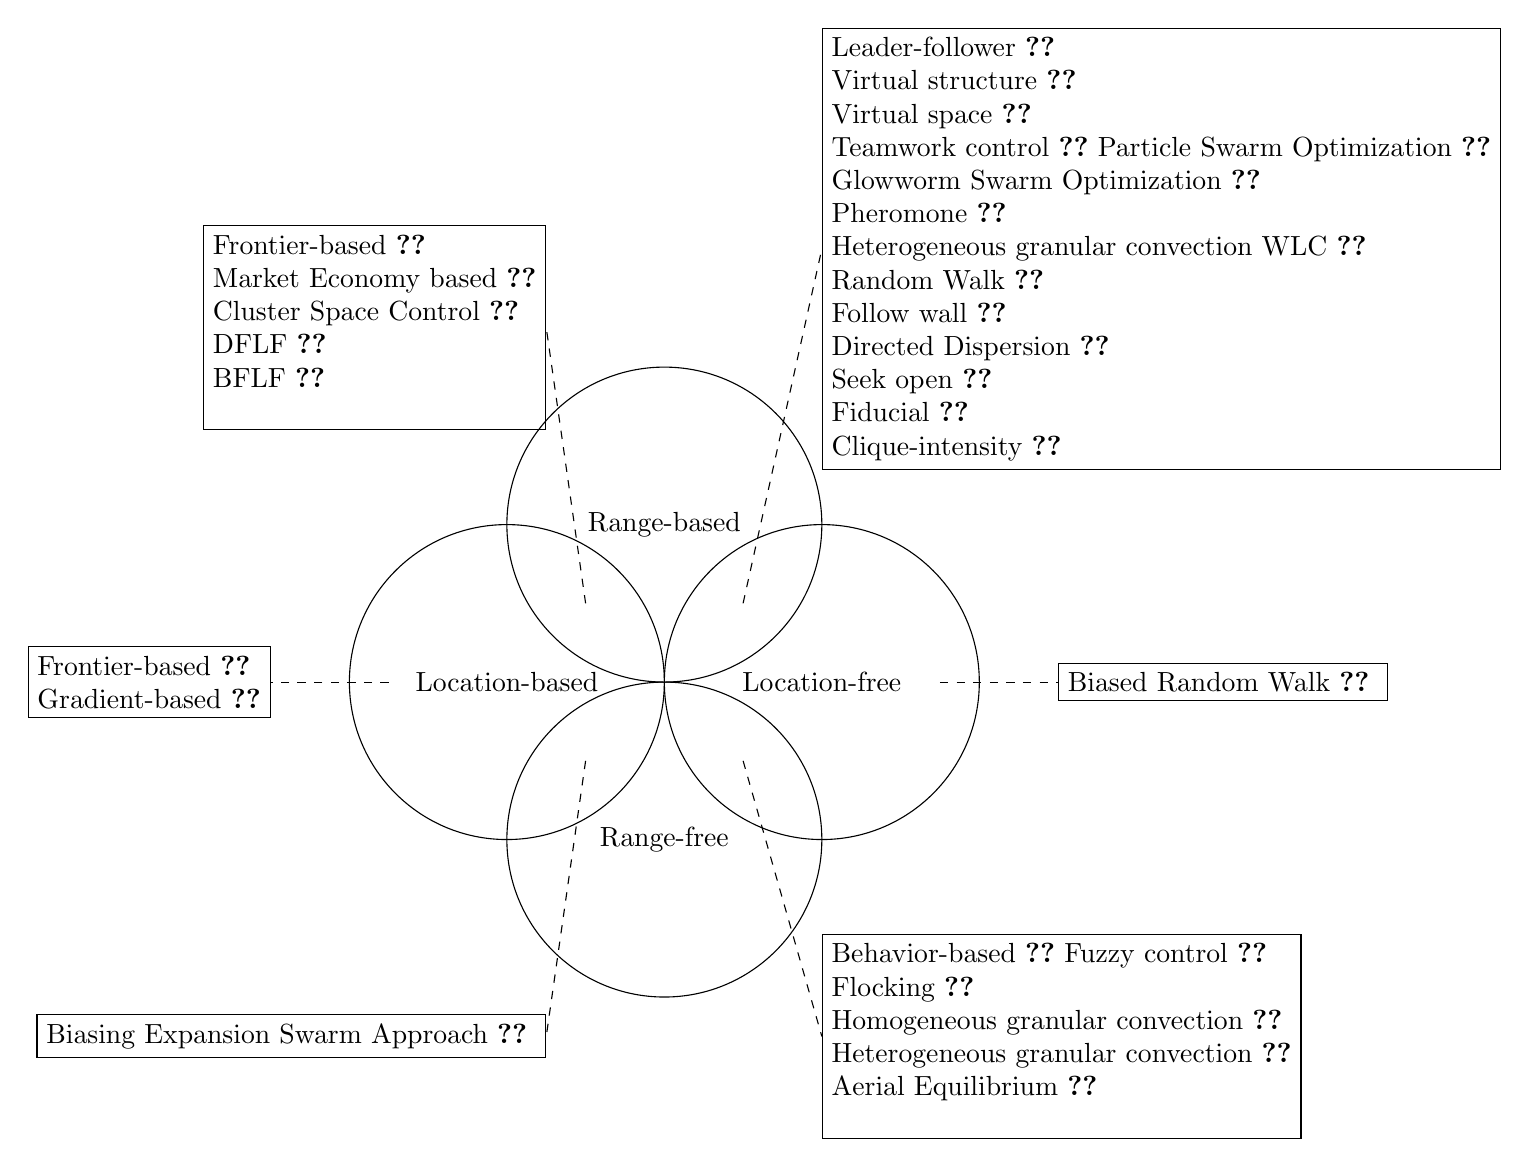
\begin{tikzpicture}
			% standard figures
			\draw \loclb node [text=black] {Location-based};
			\draw \loclf node [text=black] {Location-free};
			\draw \locrb node [text=black] {Range-based};
			\draw \locrf node [text=black] {Range-free};

			% Range-based location-free
			\draw[dashed,-] (1,1) -- (2,5.5) node[anchor=north west] {};
			\node[draw,align=left,anchor=west] at (2,5.5) {
				Leader-follower \ref{sec:Formation}\\
				Virtual structure \ref{sec:Formation}\\
				Virtual space \ref{sec:Formation}\\
				Teamwork control \ref{sec:Formation}
				Particle Swarm Optimization \ref{sec:Localization}\\
				Glowworm Swarm Optimization \ref{sec:Localization}\\
				Pheromone \ref{sec:CollectiveTransport}\\
				Heterogeneous granular convection WLC \ref{sec:CollectiveTransport}\\
				Random Walk \ref{sec:Dispersion}\\
				Follow wall \ref{sec:Dispersion}\\
				Directed Dispersion \ref{sec:Dispersion}\\
				Seek open \ref{sec:Dispersion}\\
				Fiducial \ref{sec:Dispersion}\\
				Clique-intensity \ref{sec:Dispersion}
			};

			% Range-free, location-free
			\draw[dashed,-] (1,-1) -- (2,-4.5) node[anchor=north west] {};
			\node[draw,align=left,anchor=west] at (2,-4.5) {
				Behavior-based \ref{sec:Formation}
				Fuzzy control \ref{sec:Formation}\\
				Flocking \ref{sec:CollectiveTransport}\\
				Homogeneous granular convection \ref{sec:CollectiveTransport}\\
				Heterogeneous granular convection \ref{sec:CollectiveTransport}\\
				Aerial Equilibrium \ref{sec:CollectiveTransport}\\
				%Virtual Pheromone \ref{sec:Path-planning}\\
				%Cardinality \ref{sec:Path-planning}
			};

			% location-free
			\draw[dashed,-] (3.5,0) -- (5,0) node[anchor=north west] {};
			\node[draw,align=left,anchor=west] at (5,0) {
				Biased Random Walk \ref{sec:Localization}
			};

			% location-based
			\draw[dashed,-] (-3.5,0) -- (-5,0) node[anchor=north west] {};
			\node[draw,align=left,anchor=east] at (-5,0) {
				Frontier-based \ref{sec:Exploration}\\
				Gradient-based \ref{sec:Localization}
			};

			% Range-free, location-based
			\draw[dashed,-] (-1,-1) -- (-1.5,-4.5) node[anchor=north west] {};
			\node[draw,align=left,anchor=east] at (-1.5,-4.5) {
				Biasing Expansion Swarm Approach \ref{sec:Localization}
			};

			% Range-based, location-based
			\draw[dashed,-] (-1,1) -- (-1.5,4.5) node[anchor=north west] {};
			\node[draw,align=left,anchor=east] at (-1.5,4.5) {
				Frontier-based \ref{sec:Exploration}\\
				Market Economy based \ref{sec:Exploration}\\
				Cluster Space Control \ref{sec:CollectiveTransport}\\
				DFLF \ref{sec:Dispersion}\\
				BFLF \ref{sec:Dispersion}\\
				%Artificial Bee Colony \ref{sec:Path-planning}\\
				%Multihop Communication \ref{sec:Path-planning}\\
				%Genetic Programming \ref{sec:Path-planning}
			};

			% Range-based
			%\draw[dashed,-] (0,3) -- (0,4.5) node[anchor=north west] {};
			%\node[draw,align=left,anchor=south] at (0,4.5) {

			%};

			% Range-free
			%\draw[dashed,-] (0,-3) -- (0,-4.5) node[anchor=north west] {};
			%\node[draw,align=left,anchor=north] at (0,-4.5) {
			
			%};
		\end{tikzpicture}
		\caption{Overview of Algorithms}
    \end{figure}

In the previous sections, we reviewed the main problems found in the field of robotic swarms.
However, these problems often overlap.
This is because most of the problems found in robotic swarms often consist of multiple different problems.
We focused on each main problem, highlighting the communication methods of every solution and properties of these communication methods.
We summarize these properties in a Venn-diagram in figure~\ref{fig:AlgorithmsOverview}, allowing for a compact overview of these solutions.
The algorithms we discussed in previous sections provide useful insight, from which we can derive several conclusions.
Together with the Venn-diagram, we explain how we came to these conclusions.\\
\\
\emph{Location-based} approaches keep track of some kind of map in such a way that the exact location of each swarm robot is accurately known.
Because of this, location-based approaches are often able to act efficiently and remove redundancy.
However, a couple of drawbacks can be defined.\\
\\
If an algorithm is \emph{location-based} and \emph{range-based}, the robots can create some kind of ad-hoc network to have global communication possibilities.
This global communication is very useful for exact orders and robot movement.
But, such an ad-hoc network has a limited range.
So, robots in the swarm can not split up from the rest of the groups to work outside this range.
This takes away one of the great possibilities of robotic swarms and could decrease performance.\\
\\
A robotic swarm can also accept that they do not have global communication.
Then, they can only share their map knowledge or location history with their neighbors, which will decrease performance.\\
\\
In \emph{location-based} and \emph{range-free} algorithms, the robots can communicate via some central base, but not locally. 
This can increase performance dramatically, because redundancy in communication can be removed completely.
This is caused by the fact that every robot has access to all location information of all robots.
However, this will result in very low scalability, since the reliability of the central communication is entirely dependent on the capacity of the central base.\\

\emph{Location-free} approaches do not keep track of a map and are only able to determine some kind of relative position to each.
Alternatively they do not keep track of locations at all.
This means they are able to optimally adapt to dynamic environments and can be implemented in low-level robots with cheap sensors.\\

When an algorithm is both \emph{location-free} and \emph{range-free}, there generally exists no form of coordination.
These algorithms are called collective algorithms and are often based on stochastic parameters.
These robots all have distributed algorithms, but are often heterogeneous to carry out different tasks.
These algorithms are often highly scalable, because of the low communication overhead and cheap robots. 
Because they are highly scalable, many robots can exist in a swarm, and will eventually execute a task faster than a single robot.\\

The majority of the algorithms that we discuss are \emph{location-free} and \emph{range-based}.
The main reason for this is that the algorithms mentioned in this category are very often highly scalable, have great performance and can be implemented with very simple robots.
The difference with \emph{range-free} algorithms however is that in \emph{range-based} algorithms there exists some form of local communication.
This can increase the efficiency of such an algorithm dramatically, because the versatility of the swarm increases.
The robots can for example choose to stay together and share the information they get from their sensors, but can also choose to spread out in different groups to divide tasks depending on sensor input.
Because these algorithms are so versatile, they are well-suited for many different real-life applications.\\

We would like to emphasize that there are some problems in robotic swarms, which we did not discuss in this survey.
One such a problems is the surveillance problem, which efficiently tries to patrol a certain area.
Another problem is the mapping problem, which tries to achieve collaborative mapping using robotic swarms.
The reason we did not include these problems is because these are mostly all composite problems, of which we already have described their subproblems.
Therefore we believe that these section would create a lot of redundancy and their contribution would be limited.
Composite problems are closer to the application field of robotic swarms.
For future research, we suggest to put more focus on the application aspect of robotic swarms.

